\documentclass[../main.tex]{subfiles}
\begin{document}
	
	\section{Lista 1}
	\begin{exercicio}{1}
		Seleção de exercícios da Seção 14.4 do Apostol Cálculo 1.
		\begin{itemize}
			\item Resolver os Exercícios de 1 ao 6 tanto manualmente quanto utilizando recurso CAS.
			\item Resolver o exercício 7 e exemplificar computacionalmente utilizando recurso CAS.
			\item Resolver os Exercícios de 8 ao 11 tanto manualmente quanto utilizando recurso CAS.
		\end{itemize}
	\end{exercicio}
	\begin{solucao}
		\begin{itemize}
			\item 
			\item Note que, tirando o módulo, temos
			\begin{align*}
				\|F(t)\|^2 &=\frac{4t^2}{(1+t^2)^2}+\frac{1-2t^2+t^4}{(1+t^2)^2}+\frac{(1+t^2)^2}{(1+t^2)^2}\\
				&=\frac{1+2t^2+t^4}{(1+t^2)^2}+1\\
				&=2
			\end{align*}
			Assim,
			\begin{align*}
				\|F(t)\|^2=2
				&\Rightarrow \|F(t)\|=\sqrt{2}\\
				&\Rightarrow \langle F(t), F(t) \rangle =\sqrt{2}\\
				&\Rightarrow (\langle F(t), F(t) \rangle)'=0\\
				&\Rightarrow \langle F'(t), F(t) \rangle + \langle F(t), F'(t) \rangle = 0\\
				&\Rightarrow \langle F'(t), F(t) \rangle = 0\\
				&\Rightarrow F'(t) \perp F(t)
			\end{align*}
			Como, pelas contas, $F'(t)$ é sempre ortogonal a $F(t)$, o ângulo $\theta$ entre eles é constante, sendo $\theta=\pi/2$.
			
			Para representação em animação, podemos plotar o círculo representado por $F(t)$, e o vetor tangente, que seria sua derivada em cada ponto.
			
			\begin{center}
				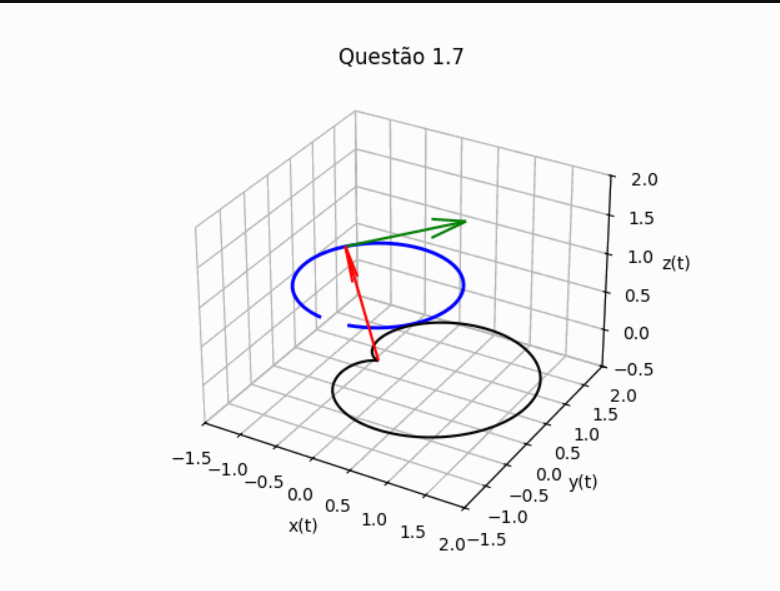
\includegraphics[width=0.25\textwidth]{imagens/lista01/picture_lista01_q01_item07.png}
				\captionof{figure}{Uma imagem da animação da parametrização $F(t)$}
			\end{center}
			\item 
		\end{itemize}
	\end{solucao}
	
	\begin{exercicio}{2}
		Encontrar uma curva (parametrizada) $\alpha(t)\colon t\in I\to \mathbb{R}^2$, cujo traço seja o círculo $x^2+y^2=1$, de maneira que $t$ percorra o círculo no sentido anti-horário e tenhamos $\alpha(0)=(0,1)$. Faça o desenho em um sistema CAS, incluindo a animação do vetor tangente percorrendo a curva.
	\end{exercicio}
	\begin{solucao}
		Para $\alpha(0)=(0,1)$, é possível $\alpha(t)=(\sin(t),\cos(t))$ ou $\alpha(t)=(-\sin(t), \cos(t))$. No entanto, para percorrer no sentido anti-horário, $x$ e $y$ devem ser decrescentes para $t\in [0,\tfrac{\pi}{2}]$. Portanto, devemos parametrizar a curva com $\alpha$, tal que $\alpha(t)=(-\sin(t), \cos(t))$.
		
		Outra forma de definir $\alpha\colon I\to \mathbb{R}^2$ seria saber que, para $\beta(t)=(\cos(t), \sin(t))$, temos sentido anti-horário com $\beta(0)=(1,0)$. Então, basta fazer uma translação do domínio em $\tfrac{\pi}{2}$, sendo $\alpha$ uma reparametrização dada por $\alpha(t)=\beta(t-\tfrac{\pi}{2})$, ou seja $\alpha(t)=(-\sin(t),\cos(t))$.
		
		Para a animação, basta plotar um cículo e o vetor tangente, variando o valor de $t$.
		
		\begin{center}
			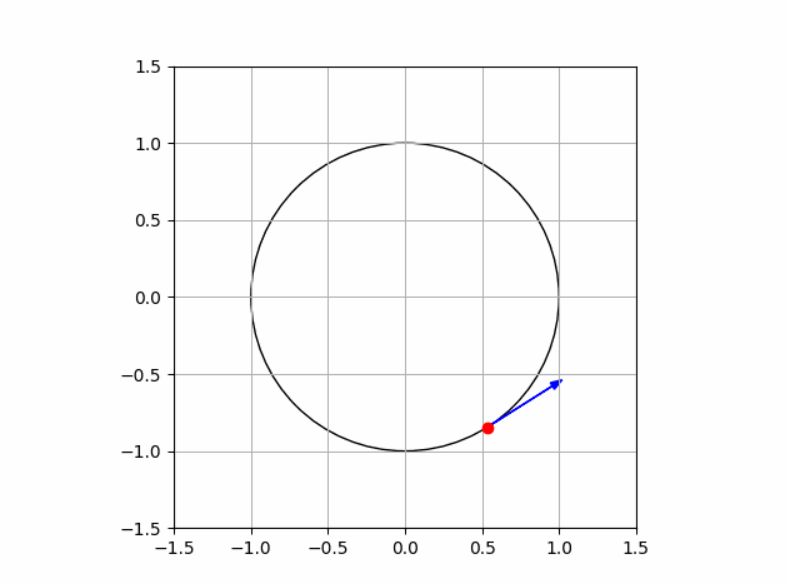
\includegraphics[width=0.25\textwidth]{imagens/lista01/picture_lista01_q02.png}
			\captionof{figure}{Uma imagem da animação da parametrização $\alpha$}
		\end{center}
	\end{solucao}
	
	\begin{exercicio}{3}
		A \textit{limaçon} (ou caracol de Pascal) é a curva parametrizada
		\[
		\gamma(t)=\bigg((1+2\cos(t))\cos(t), (1+2\cos(t))\sin(t)\bigg), t\in \mathbb{R}
		\]
		Faça o desenho desta curva num sistema CAS. Observe que o ponto $(0,0)$ pertence ao traço da curva, e ache o vetor tangente nesse ponto.
	\end{exercicio}
	\begin{solucao}
		O vetor tangete ao ponto $(0,0)$ foi encontrado da seguinte forma:
		\begin{align*}
			(0,0)=((1+2\cos(t))\cos(t),(1+2\cos(t))\sin(t))
			&\Rightarrow \begin{cases}0=(1+2\cos(t))\cos(t) \\0=(1+2\cos(t))\sin(t) \end{cases}\\
			&\Rightarrow 0=1+2\cos(t)\\
			&\Rightarrow \cos(t)=-\frac{1}{2}\\
			&\Rightarrow \begin{cases} t_{1}=\frac{2\pi}{3} \\ t_{2}=\frac{4\pi}{3} \end{cases}
		\end{align*}
		Assim, basta plotar a função $\gamma$ e os vetores tangentes no ponto $(0,0)$.
		\begin{center}
			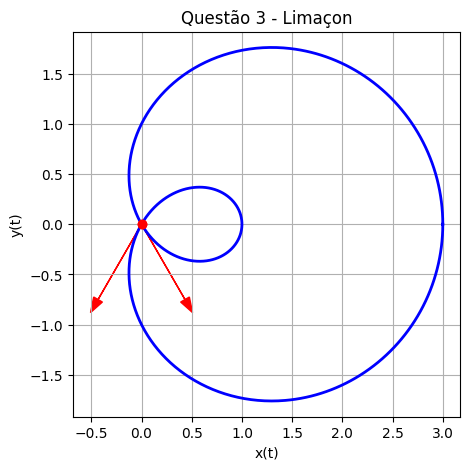
\includegraphics[width=0.25\textwidth]{imagens/lista01/picture_lista01_q03.png}
			\captionof{figure}{Limaçon com vetores tangentes no ponto $(0,0)$}
		\end{center}
	\end{solucao}
	
	\begin{exercicio}{7}
		Escolha uma curva "famosa" de sua preferência, desenhe uma animação da curva e seus vetores tangentes par auma dada parametrização e discuta a conveniência de uma nova parametrização ao avaliar a maneira como a trajetória está sendo percorrida. Referência na web de curvas famosas: https://mathshistory.st-andrews.ac.uk/Curves/.
	\end{exercicio}
	\begin{solucao}Parametrização do cardioide. Suas reparametrizações foram feitas com as seguintes funções:
		\begin{itemize}
			\item $f_{1}(x)=-x$
			\item $f_{2}(x)=x-\frac{\pi}{2}$
			\item $f_{3}(x)=2x$
		\end{itemize}	
		A primeira é conveniente, caso seja necessário alterar o sentido pelo qual a parametrização ocorre.
		\begin{center}
			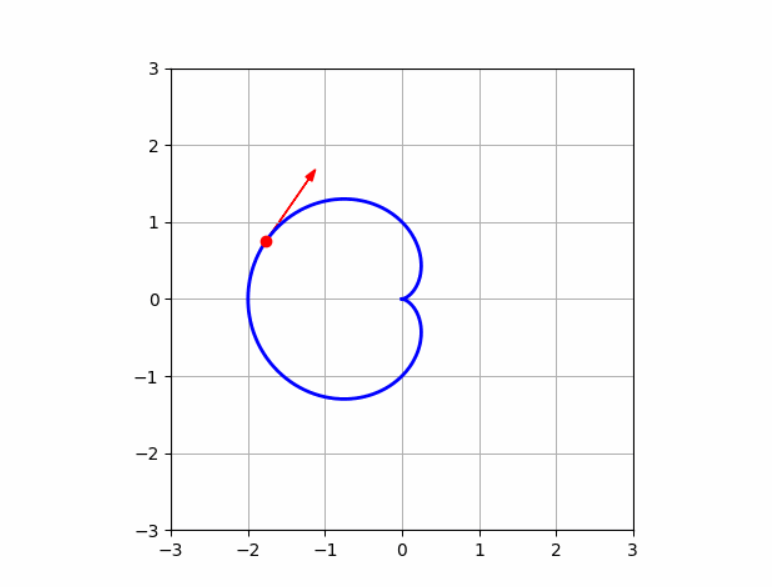
\includegraphics[width=0.25\textwidth]{imagens/lista01/picture_lista01_q07_item01.png}
			\captionof{figure}{Cardioide com reparametrização $f_{1}$}
		\end{center}
		
		A segunda é conveniente, caso seja necessário alterar o momento inicial da parametrização.
		\begin{center}
			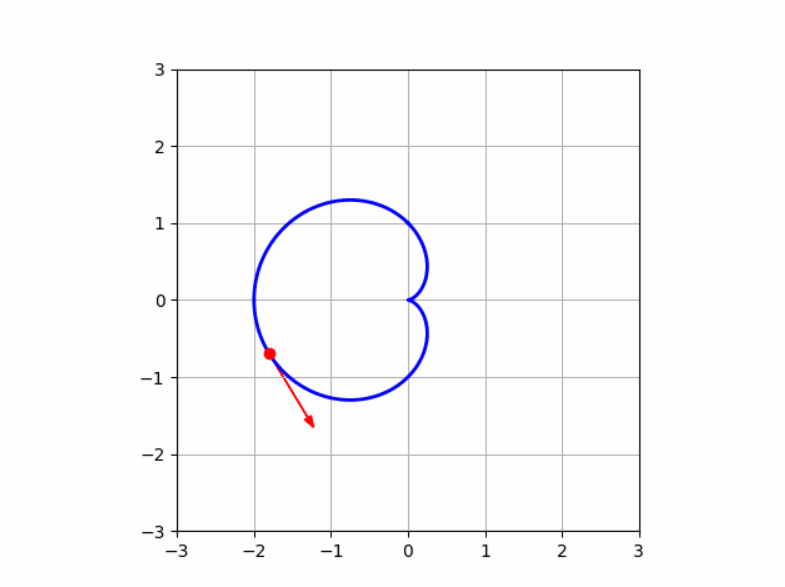
\includegraphics[width=0.25\textwidth]{imagens/lista01/picture_lista01_q07_item02.png}
			\captionof{figure}{Cardioide com reparametrização $f_{2}$}
		\end{center}
		
		O terceiro é conveniente, caso seja desejado alterar a valocidade com a qual a parametrização ocorre (note que, além de estar visivelmente mais rápido, o vetor tangente está maior).
		
		\begin{center}
			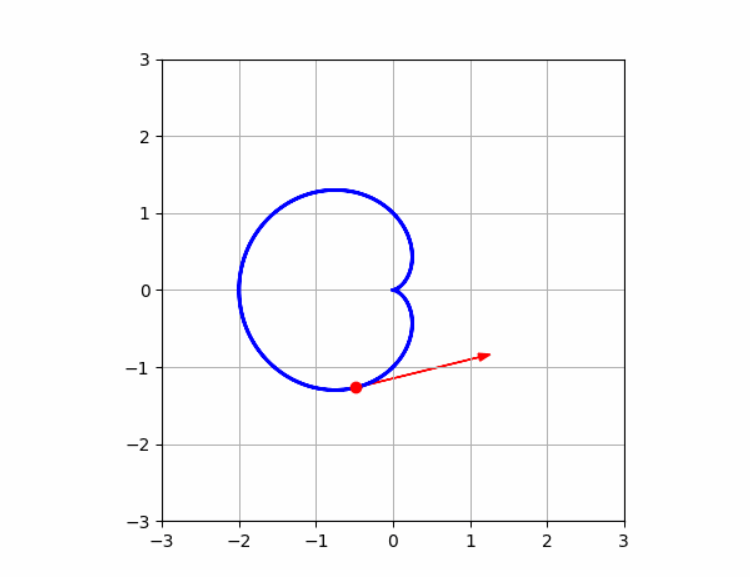
\includegraphics[width=0.25\textwidth]{imagens/lista01/picture_lista01_q07_item03.png}
			\captionof{figure}{Cardioide com reparametrização $f_{3}$}
		\end{center}
		A plotagem foi feita em SimPy.
	\end{solucao}
	
	\begin{exercicio}{9}
		Seja $\alpha\colon I\to \mathbb{R}^2$ uma curva regular. Prove que $\|\alpha'(t)\|$ é constante se, e somente se, para cada $t\in I$, o vetor $\alpha''(t)$ é ortogonal a $\alpha'(t)$.
	\end{exercicio}
	\begin{solucao}
		Vamos provar a ida. Se $\|\alpha'(t)\|$ é constante, temos que  
		\begin{align*}
			\exists c\in \mathbb{R}, \|\alpha'(t)\|=c, \forall t\in I
			&\Rightarrow \exists c\in \mathbb{R}, \langle \alpha'(t), \alpha'(t) \rangle=c^2\\
			&\Rightarrow  (\langle \alpha'(t), \alpha'(t) \rangle)'=(c^2)'=0\\
			&\Rightarrow \langle \alpha''(t), \alpha'(t) \rangle + \langle \alpha'(t), \alpha''(t) \rangle =0\\
			&\Rightarrow \langle \alpha''(t), \alpha'(t) \rangle=0
		\end{align*}
		Logo, $\|\alpha''(t)\|$ e $\|\alpha'(t)\|$ são ortogonais, $\forall t\in I$.
		
		Vamos provar a volta. Se $\|\alpha''(t)\|$ e $\|\alpha'(t)\|$ são ortogonais, $\forall t\in I$, temos que
		\begin{align*}
			\langle \alpha''(t), \alpha'(t) \rangle=0
			&\Rightarrow \exists c\in \mathbb{R}, \langle \alpha'(t), \alpha'(t) \rangle=c, \forall t\in I\\
			&\Rightarrow \exists c\in \mathbb{R}, \|\alpha'(t)\|=c, \forall t\in I\\
		\end{align*}
		Logo, $\|\alpha'(t)\|$ é constante.
		
		Com isso, concluímos a prova.
	\end{solucao}
\end{document}
